
\documentclass[12pt]{article}

% Layout.
\usepackage[top=1in, bottom=0.75in, left=1in, right=1in, headheight=1in, headsep=6pt]{geometry}

% Fonts.
\usepackage{mathptmx}
\usepackage[scaled=0.86]{helvet}
\renewcommand{\emph}[1]{\textsf{\textbf{#1}}}

% TiKZ.
\usepackage{tikz, pgfplots}
\usetikzlibrary{calc}
\pgfplotsset{compat = newest}
 
\pgfplotsset{my style/.append style={axis x line=middle, axis y line=
middle, xlabel={$x$}, ylabel={$y$}, axis equal }}

% Misc packages.
\usepackage{amsmath,amssymb,latexsym}
\usepackage{graphicx}
\usepackage{array}
\usepackage{xcolor}
\usepackage{multicol}

% Commands to set various header/footer components.
\makeatletter
\def\doctitle#1{\gdef\@doctitle{#1}}
\doctitle{Use {\tt\textbackslash doctitle\{MY LABEL\}}.}
\def\docdate#1{\gdef\@docdate{#1}}
\docdate{Use {\tt\textbackslash docdate\{MY DATE\}}.}
\def\doccourse#1{\gdef\@doccourse{#1}}
\let\@doccourse\@empty
\def\docscoring#1{\gdef\@docscoring{#1}}
\let\@docscoring\@empty
\def\docversion#1{\gdef\@docversion{#1}}
\let\@docversion\@empty
\makeatother

% Headers and footers layout.
\makeatletter
\usepackage{fancyhdr}
\pagestyle{fancy}
\fancyhf{} % Clears all headers/footers.
\lhead{\baselineskip 30pt
%\emph{\@doctitle\hfill\@docdate}
\emph{\@docdate\hfill\@doctitle}
\ifnum \value{page} > 1\relax\else\\
\emph{Name: \rule{3.5in}{1pt}\hfill \@docscoring}\fi}
\rfoot{\emph{\@docversion}}
\lfoot{\emph{\@doccourse}}
\cfoot{\emph{\thepage}}
\renewcommand{\headrulewidth}{0pt}%
\makeatother

% Paragraph spacing
\parindent 0pt
\parskip 6pt plus 1pt

% A problem is a section-like command. Use \problem{5} to
% start a problem worth 5 points.
\newcounter{probcount}
\newcounter{subprobcount}
\setcounter{probcount}{0}
\newcommand{\problem}[1]{%
\par
\addvspace{4pt}%
\setcounter{subprobcount}{0}%
\stepcounter{probcount}%
\makebox[0pt][r]{\emph{\arabic{probcount}.}\hskip1ex}\emph{[#1 points]}\hskip1ex}
\newcommand{\thesubproblem}{\emph{\alph{subprobcount}.}}

% Subproblems are an enumerate-like environment with a consistent
% numbering scheme. 
% Use \begin{subproblems}\item...\item...\end{subproblems}
\newenvironment{subproblems}{%
\begin{enumerate}%
\setcounter{enumi}{\value{subprobcount}}%
\renewcommand{\theenumi}{\emph{\alph{enumi}}}}%
{\setcounter{subprobcount}{\value{enumi}}\end{enumerate}}

% Blanks for answers in normal and math mode.
\newcommand{\blank}[1]{\rule{#1}{0.75pt}}
\newcommand{\mblank}[1]{\underline{\hspace{#1}}}
\def\emptybox(#1,#2){\framebox{\parbox[c][#2]{#1}{\rule{0pt}{0pt}}}}

% Misc.
\renewcommand{\d}{\displaystyle}
\newcommand{\ds}{\displaystyle}
\def\bc{\begin{center}}
\def\ec{\end{center}}
\def\be{\begin{enumerate}}
\def\ee{\end{enumerate}}


\doctitle{Math 251: Quiz 2}
\docdate{Sept 8, 2022}
\doccourse{UAF Calculus I}
\docversion{v-1}
\docscoring{\blank{0.8in} / 25}
\begin{document}
%\textbf{Please circle your instructor's name:} \hfill Leah Berman  \hfill   Jill Faudree\\

There are 25 points possible on this quiz. No aids (book, calculator, etc.)
are permitted.  {\bf Show all work for full credit.}

\begin{enumerate}
\item (6 points) In the unit circle below, the details for Quadrant 1 have been provided. Fill in the remaining details for Quadrant 3. (You must fill in \emph{FIVE} boxes indicating angles in radians and \emph{FIVE} ordered pairs of points.\\
\begin{tikzpicture}[scale=5,cap=round,>=latex]  
        % draw the coordinates
        \draw[->] (-1.5cm,0cm) -- (1.5cm,0cm) node[right,fill=white] {$x$};
        \draw[->] (0cm,-1.1cm) -- (0cm,1.4cm) node[left,fill=white] {$y$};
        % draw the unit circle
        \draw[thick] (0cm,0cm) circle(1cm);
	% draw radii, points, and angles in degrees
        \foreach \x in {0,30,45,60,90,180,210,225,240,270} {
                % lines from center to point
                \draw[black] (0cm,0cm) -- (\x:1cm);
                % dots at each point
                \filldraw[black] (\x:1cm) circle(0.4pt);
                % draw each angle in degrees
                \draw (\x:0.5cm) node[fill=white] {$\x^\circ$};
                 }       
 % draw each angle in Quadrant 1 in radians
        \foreach \x/\xtext in {
        	    0/0,
            30/\frac{\pi}{6},
            45/\frac{\pi}{4},
            60/\frac{\pi}{3},
            90/\frac{\pi}{2}}
            \draw (\x:0.85cm) node[fill=white] {$\xtext$};
 % draw answer boxes and blank ordered pairs in Quadrant 3
 	\foreach \x in {210,225,240,270}{
		\draw (\x:0.8cm) node[fill=white] {\mbox{\framebox(22,22){}}};
		\draw (\x:1.25cm) node[fill=white] {$\left(\quad\quad\quad, \quad \quad \quad\right)$};
	}
% draw 180 separately so it looks good
\draw (180:0.8cm) node[fill=white] {\mbox{\framebox(22,22){}}};
\draw (175:1.3cm) node[fill=white] {$\left(\quad\quad, \quad \quad \right)$};

% ordered pairs of points in Quadrant 1	
        \foreach \x/\xtext/\y in {
            30/\frac{\sqrt{3}}{2}/\frac{1}{2},
            45/\frac{\sqrt{2}}{2}/\frac{\sqrt{2}}{2},
            60/\frac{1}{2}/\frac{\sqrt{3}}{2}}
                \draw (\x:1.25cm) node[fill=white] {$\left(\xtext,\y\right)$};
        % draw the horizontal and vertical coordinates
        % the placement is better this way
        \draw 
              (1.25cm,0cm)  node[above=1pt] {$(1,0)$}
              (0cm,1.25cm)  node[fill=white] {$(0,1)$};
    \end{tikzpicture}
    
 \item (4 points) Evaluate the trigonometric functions. Assume all angles are in radians. Simply your answers.\\
 
 {\large{$\sin(3 \pi/2)=$}} \hfill {\large{$\tan(7\pi/6)=$}}\hspace{1in}\quad
 \vspace{.2in}
\newpage
\thispagestyle{plain}
\vspace*{-2cm}
\item (5 points) For five seconds, the position of a moose running down Yukon Drive is modeled by $d(t)=t^2,$ where $t$ is time in seconds and $d$ is distance in meters. Find the average velocity of the moose between $t=3$ and $t=5.$ Include units with your answer.
\vspace{1in}

\item(10 points) Let $g(x)=\frac{12}{x+1}.$ Observe that $P(1,6)$ is a point on the graph of $g(x).$
\begin{enumerate}
\item Find the slope of the secant line passing through $P$ and the point $Q(3,g(3)).$ 
\vfill

%\item Write an equation of the line between the points $P$ and $Q.$
%
%\vfill

\item The table below lists the slope of the secant line passing through the point $P$ and the point $Q(x, f(x))$ for several values of $x.$ 

\begin{tabular}{l || c|c|c|c|c|c|c}
x&0.9&0.99&0.999&1&1.001&1.01&1.1\\
\hline
g(x)&6.3157&6.0302&6.0030&6&5.9970&5.9701&5.7143\\
\hline
$m_{sec}$&-3.1579&-3.0151&-3.0015&&-2.9985&-2.9851&-2.8571
\end{tabular}

\vskip 0.5cm
Use the information in the table to estimate the slope of the tangent line to $g(x)$ at the point $P(1,6).$
\vfill


\item Use the slope from part (b) above to write an equation of the tangent line to $g(x)$ at point $P(1,6).$

\vfill

\item \quad 

\begin{multicols}{2}
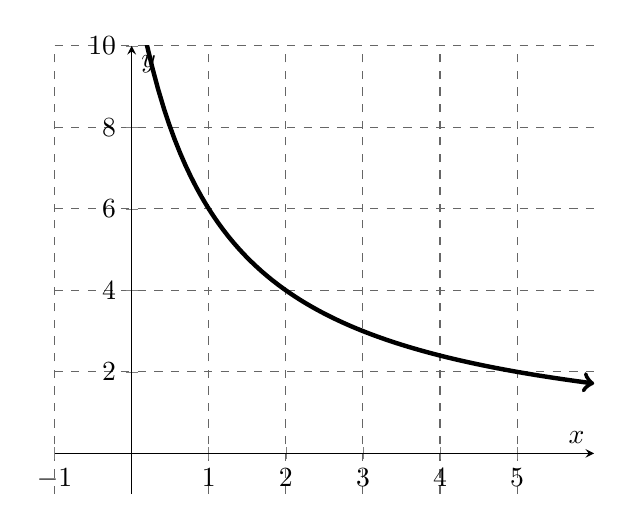
\begin{tikzpicture}
 \begin{axis}[
    xmin = -1, xmax = 6,
    ymin = -1, ymax = 10, xtick={-1,0,...,5}, ytick={-2,0,...,10},
    grid=both, grid style={ thin, black!60, dashed},axis x line=middle, axis y line=
middle, xlabel={$x$}, ylabel={$y$}]
    \addplot[ultra thick, <->,samples=100,
        domain = -1:6,
    ] {12/(x+1)};
    %\addplot[thick,->] coordinates {(-1,0) (6,0)};
\end{axis}
\end{tikzpicture}

Left is a sketch of the graph of $$f(x)=\displaystyle{\frac{12}{x+1}}.$$ \\
Sketch and label the \emph{tangent} line to the graph at the point $P(1,6).$\\
Sketch and label the \emph{secant} line between $P(1,6)$ and $Q(3,g(3)).$
\end{multicols}
\end{enumerate}
\end{enumerate}	
\end{document}